%================================================
%	载入文档类,配置文档类选项
%================================================

\documentclass[%truetimes,
               %print, 
               %timesmath,
               amsthm,
              ]{xjtubsc}

% truetimes 选项会使用windows 自带的 Times New Roman 字体,否则使用 TeX 发行版的 Times 字体,几乎没有区别,肉眼凡胎看不出差别。开启 truetiems 选项必须使用 XeLaTeX 编译。否则关闭 truetiems。推荐开启。且推荐使用 XeLaTeX 编译。

% print 选项会去除超链接的颜色。以供打印。根据需求开启。

% timesmath 将会使用 Times 风格的数学字体,以使与正文的 Times 英文字体更加搭配。根据需求开启。

% amsthm 将会调用 amsthm 宏包及 thmtool 宏包,而且配置好了常用的 定义、定理、证明等环境。推荐开启。

%================================================
%	加载宏包、配置宏包选项、自定义命令等
%================================================


\usepackage{xjtupackages} % 这是对常用宏包的一个打包,供初级用户使用。如需在此基础上载入其他宏包,请先阅读 xjtupackages.sty 文件,以免造成冲突。

\graphicspath{{figures/},{figs/}} % 仿照此格式设置图片路径,需要graphicx支持(xjtupackages中已载入)

\DeclareMathOperator{\coker}{coker}
\newcommand\abs[1]{\left\lvert#1\right\rvert}
\newcommand*\diff{\mathop{}\!\mathrm{d}}


\begin{document}
%================================================
%	下面填写基本信息
%================================================

% 以下三项是必须的。
\author{王鸿鑫、秦雨果、郝运}{Hongxin WANG, Yuguo QIN, Yun HAO}	%	作者{中文}{英文}
\title{西安交通大学理学学士毕业论文 \LaTeX{} 模板示例文件}{Example of \LaTeX{} Template for Bachelor of Science Thesis in XJTU}	%	题目{中文}{英文}
\advisor{王鸿鑫、秦雨果、郝运}{Hongxin WANG, Yuguo QIN, Yun HAO}	%	导师{中文}{英文}

% 如果不希望 \LaTeX{} 生成任务书、评议书、意见书、答辩结果,下面的信息可以不填。这里内容换行请用\xjtunewline
\college{数学与统计}	%	学院
\department{数学}	%	专业(系)
\class{理科数学 91}	%	班级
\place{西安交通大学}	%	毕设地点
\bdate{2012/12/21}	% 开始时间,格式为:年/月/日
\edate{2013/2/15}	% 结束时间,格式为:年/月/日

\begin{INFObackground} % 课题的背景、意义及培养目标 

在微分几何中,高斯-博内定理(亦称高斯-博内公式)是关于曲面的图形(由曲率表征)和拓扑(由欧拉示性数表征)间联系的一项重要表述。\xjtunewline
它是以卡尔·弗里德里希·高斯和皮埃尔·奥西安·博内命名的,前者发现了定理的一个版本但从未发表,后者1848年发表了该定理的一个特例。\xjtunewline
这里换行请用\textbackslash xjtunewline

\end{INFObackground}

\begin{INFOdata} % 设计(论文)的原始数据与资料


\end{INFOdata}

\begin{INFOtask} % 课题的主要任务


\end{INFOtask}

\begin{INFOrequirement} % 课题的主要任务


\end{INFOrequirement}

\begin{INFOsubmit} % 课题的主要任务


\end{INFOsubmit}

\begin{INFOreference} % 课题的主要任务


\end{INFOreference}

%================================================
%	正文前
%================================================
\frontmatter

\extrapages % 用于输出任务书、评议书、意见书、答辩结果。如果不希望 \LaTeX{} 生成任务书、评议书、意见书、答辩结果,可以注释掉此句。

\begin{abstractcn} % 中文摘要
这是 \emph{西安交通大学理学学士毕业论文 \LaTeX{} 模板} 的示例文件,目标使用者为有 \LaTeX{} 经验的同学。如果毫无 \LaTeX{} 使用经验,强烈建议认真学习入门教程\footnote{比如:?、?和?}~24~小时后再使用。使用 LaTeX 模板可减少很多排版上的烦恼,但如果使用不当亦会增加痛苦。

本模板尚未得到官方的认可,如有任何关于其是否被认可的问题,请咨询教务员。我们会尽我们最大的努力使得该模板被官方接受。

如有任何关于模板使用的问题,可以向作者咨询,但不一定能及时得到答复。如果需要 24 小时之内答复,可向作者支付 \emph{五毛} 人民币每次(此技术支持对西安交通大学数学拔尖班同学免费)。

\end{abstractcn}

\keywordscn{中文;摘要;关键词} % 中文关键词

\begin{abstracten} % 英文摘要

This is the \emph{\LaTeX{} template for Bachelor of Science Thesis in Xi'an Jiaotong University} with expected users who have some experience with \LaTeX{}. If you have no experience with \LaTeX{}, we SUGGEST that you learn a basic tutorial on \LaTeX{} for more than 24 hours before using the template. Proper use will free you from the worries of typography of your thesis, however, improper use will definitely increasing your pain.

This template has no authorization from the dean's office. If you have any question with respect to the legality of the template, please consult the dean's office of your department or school.

\end{abstracten}

\keywordsen{English; Abstract; Key Words} % 英文关键词

\tableofcontents % 生成目录


%================================================
%	正文
%================================================
\mainmatter


\section{简介}
这是西安交通大学理学学士毕业论文 \LaTeX{} 模板。推荐使用 \hologo{XeLaTeX} 编译,可以使用 \hologo{pdfLaTeX} 编译。
经测试可以在 Windows、GNU/linux、Mac OS 平台上利用 MikTeX、TeXLive、MacTeX 等发行版本正常编译\footnote{需要系统中安装有中易宋、黑、楷、仿宋四款字体,这在中文 Windows 下是默认安装的。如果需要自己配置字体,可以参考第~\ref{sec:customfont} 节的内容}。

项目地址是 \url{www.github.com/haoyun/xjtu-thesis-bsc/}。欢迎下载试用并反馈遇到的问题,如有任何建议及想法也请告诉我们。你可以发送邮件给作者,也可以到项目主页上提交 Issue。

作者及联系方式为:
\begin{center}
\begin{tabular}{lp{1em}l}
郝运&&\href{maito:haoyun_tex@163.com}{haoyun\_tex@163.com}\\ 秦雨果&&\\
王鸿鑫&&\href{maito:hongxin_w@163.com}{hongxin\_w@163.com}
\end{tabular}
\end{center}

\section{使用指南}
\subsection{准备工作}

%首先你需要安装一个 \TeX{} 发行版,比如 C\TeX{} 套装、MikTeX 套装,TeXLive 2012,MacTex 等。Windows 用户可以参考附录~\ref{append:install}。
%
%在使用之前要更新宏包:特别是 xeCJK 及其相关依赖。Windows 用户可以参考附录~\ref{append:install}。
%
%如果有特殊需求,例如使用 Times 风格的数学字体,还需安装 texgyremath 宏包。 

为了正常使用此模板,并避免不必要的麻烦,请完全安装 MikTeX(或相应的 C\TeX 套装),TeXLive、MacTex 的最新版,并在线升级\footnote{至少升级 xeCJK 宏包至最新版,如开启 timesmath 选项,请确保有 tex-gyre-math 宏包。}。Windows 用户可以参考附录~\ref{append:install}。

{\color{red}注意},为了得到更好的技术支持,强烈建议使用 \hologo{XeLaTeX} 编译。

\subsection{文档基本结构}
一个建议的工作目录结构如下\footnote{正如 \verb|example| 文件夹的结构。}:
\begin{verbatim}
    Working Dir.:
    |  GBT7714-2005NLang-UTF8-mod.bst   --- 参考文献格式
    |  main.tex                         --- 主控文档
    |  make.bat                         --- 批处理,未完成
    |  xjtubsc.cls                      --- 模板 LaTeX 文档类文件
    |
    |─figures                          --- 存放插图的文件夹
    |     |─some figures
    |
    |─pages                            --- 存放论文内容的文件夹
    |     |─the files
    |
    |─ref                              --- 存放参考文献的文件夹
          |─the refs
\end{verbatim}
其中二级目录不是必须的,而且目录名可以根据自己的喜好任选。

文档的基本结构为
\begin{verbatim}
    \documentclass{xjtubsc}
        <导言部分>
    \begin{document}
        <设置基本信息>
        \frontmatter  
            <任务书等、摘要、目录>
        \mainmatter
            <正文部分>
        \backmatter
            <附录、致谢部分>
\end{verbatim}

UTF8 编码!!!
\subsection{文档类及文档类选项}

\begin{itemize}
\item[truetimes] 选项会使用windows 自带的 Times New Roman 字体,否则使用 TeX 发行版的 Times 字体,几乎没有区别,肉眼凡胎看不出差别。开启 truetiems 选项必须使用 XeLaTeX 编译。否则关闭 truetiems。推荐开启。且推荐使用 XeLaTeX 编译。

\item[print] 选项会去除超链接的颜色。以供打印。根据需求开启。

\item[timesmath] 将会使用 Times 风格的数学字体,以使与正文的 Times 英文字体更加搭配。根据需求开启。

\item[amsthm] 选项会载入 amsthm 宏包,并配置好常用的定义定理环境。
\end{itemize}

\subsection{加载宏包}
xjtupackages.sty

\subsection{填写基本信息,生成任务书等内容}

首先必须\footnote{此处“必须”是指:是为了得到完整的摘要页面(以及可选的任务书等页面),这三项内容是必须的,如果不定义此三项内容,本模板依然正常编译,只会给出警告(Warning),而不会报错(Error)而停止编译,输出结果中保持相应位置处空白。}填写作者信息、导师信息的内容\footnote{这部分内容可以位于 \verb+\begin{document}+ 之前,也可以位于其后。}。命令格式为 \verb|\command{中文}{英文}|,如下所示:
\begin{verbatim}
    \author{作者}{Author}
    \title{题目}{Title}
    \advisor{导师}{Advisor}
\end{verbatim}


如果需要由 \LaTeX{} 生成 \emph{毕业设计(论文)任务书},\emph{毕业设计(论文)考核评议书},\emph{毕业设计(论文)评审意见书} 以及 \emph{毕业设计(论文)答辩结果} 四个表单页面,那么需要 \verb|\college|、\verb|\department|、\verb|\class|、\verb|\place|、\verb|\bdate|、\verb|\edate| 命令来定义基本信息\footnote{同样,这部分内容可以位于 \verb+\begin{document}+ 之前,也可以位于其后。},并通过 \verb|INFObackground|、\verb|INFOdata|、\verb|INFOtask|、\verb|INFOrequirement|、\verb|INFOsubmit| 以及 \verb|INFOsummit| 环境来填写任务书表单。然后使用 \verb|\extrapages| 命令来生成页面。一个简单的例子如下:
\begin{verbatim}
    \college{数学与统计}	%	学院
    \department{数学}	%	专业(系)
    \class{理科数学 91}	%	班级
    \place{西安交通大学}	%	毕设地点
    \bdate{2012/12/21}	% 开始时间,格式为:年/月/日
    \edate{2013/2/15}	% 结束时间,格式为:年/月/日
    
    \begin{INFObackground} % 课题的背景、意义及培养目标 
        这里输入内容
    \end{INFObackground}
    ……
    
    \frontmatter % 设置为正文前格式
    \extrapages % 用输出任务书、评议书、意见书、答辩结果。
\end{verbatim}
特别需要注意的是开始时间和结束时间的格式,另外,上述内容的任何一项均可不写(当然此时相应表单处空白不填)。还需要注意的是,即使不使用 \verb|\extrapages| 来排版任务书等,摘要页面的页码依然从 V \footnote{罗马数字 5。从正文开始采用阿拉伯数字页码,从 1 开始编号.}开始编号。

在定义完\verb|\author|、\verb|\title|、\verb|\advisor| 三项内容之后,开始输入中英文摘要及关键词并生成目录。示例如下:
\begin{verbatim}
    \frontmatter % 设置为正文前格式,如果已经设置则无需此命令。
    \begin{abstractcn} % 中文摘要
        中文摘要
    \end{abstractcn}
    
    \keywordscn{中文;摘要;关键词} % 中文关键词
    
    \begin{abstracten} % 英文摘要
        English Abstract.
    \end{abstracten}
    
    \keywordsen{English; Abstract; Key Words} % 英文关键词
    
    \tableofcontents % 生成目录
\end{verbatim}
注意为了正确生成目录,需要至少两次编译。

至此完成正文之前的部分。

\subsection{正文部分}

正文部分首先以 \verb|\mainmatter| 开始,以设置为正文部分的格式。

文件结构使用 \verb|\section{}|、\verb|\subsection{}|、\verb|\subsubsection{}| 来控制。而且仅支持此三层结构\footnote{当然支持 \verb|\paragraph{}|,但此很少使用,如果需要添加更深层次结构的支持,请自行 hack。模板作者建议合理安排文档结构,只有在非常罕见的情况下,四级、五级结构才是必须的。},不支持 \verb|\part{}| 和 \verb|\chapter{}|。

为了便于编写,推荐将每个 \verb|\section{}| 单独的保存为一个 \verb|.tex| 文件,然后使用 \verb|\include{foobar.tex}| 命令来插入。

注意如果插入的部分在次一级的文件目录里面,例如我们所推荐的
\begin{verbatim}
    \include{pages/foobar.tex}
\end{verbatim}
请注意 \verb|/| 的方向以及扩展名(Windows、Mac OS、Linux 下可能有所不同)。\textbf{(本段需要完善。)}

其余使用方法同基本文档类完全相同。

\subsection{参考文献}

正文完成后首先使用 \verb|\backmatter| 切换至正文后的排版格式。然后使用相应的命令来实现参考文献的排版。推荐使用 \hologo{BibTeX} 排版参考文献。一个例子如下:
\begin{verbatim}
    \backmatter % 切换至正文后版式。

    \nocite{*} % 显示未明显引用的所有文献
    \bibliographystyle{GBT7714-2005NLang-UTF8-mod} 
    % 使用 GB/T7714-2005 标准的文献格式。
    \bibliography{ref/refs} % bib 文件的为 /ref/refs.bib
\end{verbatim}
注意上面使用了 \verb|GBT7714-2005NLang-UTF8-mod.bst|,请确保工作目录下有此文件。如果想使用其他的格式(注意教务处要求),可以根据自己的喜好替换。

当然也可以使用 thebibliography 环境手工排版参考文献,一个示例如下:
\begin{verbatim}
    \begin{thebibliography}{5}
    \bibitem {}
    \end{thebibliography}
\end{verbatim}

可以用相应的工具生成符合格式的 \verb|.bib| 文件,或相应的 thebibliography 环境代码。网上有很多相应的工具,数据库一般情况下可以导出 \verb|.bib| 文件(Export Citation)。

还有一种较新的实现方式是还用 \textsc{Bib}\LaTeX{}/biber,不推荐初级用户使用。
\subsection{附录}

\subsection{高级部分}

\subsubsection{自定义字体}\label{sec:customfont}
\subsubsection{自定义宏包}
something

\section{排版效果展示}

\subsection{公式测试}
这是公式测试。公,公,公式的公,式,式,公式的式。

\begin{align}
\begin{split}\abs{I_1} &= \left\lvert \int_\Omega gRu\diff\Omega\right\rvert\\
  & \le C_3\left[\int_\Omega\left(\int_{a}^x g(\xi,t)\diff\xi\right)^2\diff\Omega\right]^{1/2}
       \times\left[\int_\Omega\left\{u^2_x+\frac{1}{k}
    \left(\int_{a}^x cu_t\diff\xi\right)^2\right\}\diff\Omega\right]^{1/2}\\
  & \le C_4\left\lvert \left\lvert f\left\lvert \widetilde{S}^{-1,0}_{a,-}W_2(\Omega,\Gamma_l)
    \right\rvert\right\rvert\left\lvert \abs{u}\overset{\circ}\to W_2^{\widetilde{A}}
    (\Omega;\Gamma_r,T)\right\rvert\right\rvert.
\end{split}\\
\begin{split}\abs{I_2} &= \left\lvert \int_{0}^T \psi(t)\left\{u(a,t)
  -\int_{\gamma(t)}^a\frac{\diff\theta}{k(\theta,t)}
  \int_{a}^\theta c(\xi)u_t(\xi,t)\diff\xi\right\}\diff t\right\rvert\\
  & \le C_6\left\lvert \left\lvert f\int_\Omega\left\lvert \widetilde{S}^{-1,0}_{a,-}
    W_2(\Omega,\Gamma_l)\right\rvert\right\rvert\left\lvert \abs{u}\overset{\circ}
    \to W_2^{\widetilde{A}}(\Omega;\Gamma_r,T)\right\rvert\right\rvert.
\end{split}\tag{\theequation$'$}
\end{align}

\[
\begin{tikzpicture}[>=triangle 60]
  \matrix[matrix of math nodes,column sep={60pt,between origins},row
    sep={60pt,between origins},nodes={asymmetrical rectangle}] (s)
  {
    &|[name=ka]| \ker f &|[name=kb]| \ker g &|[name=kc]| \ker h \\
    %
    &|[name=A]| A' &|[name=B]| B' &|[name=C]| C' &|[name=01]| 0 \\
    %
    |[name=02]| 0 &|[name=A']| A &|[name=B']| B &|[name=C']| C \\
    %
    &|[name=ca]| \coker f &|[name=cb]| \coker g &|[name=cc]| \coker h \\
  };
  \draw[->] (ka) edge (A)
            (kb) edge (B)
            (kc) edge (C)
            (A) edge (B)
            (B) edge node[auto] {\(p\)} (C)
            (C) edge (01)
            (A) edge node[auto] {\(f\)} (A')
            (B) edge node[auto] {\(g\)} (B')
            (C) edge node[auto] {\(h\)} (C')
            (02) edge (A')
            (A') edge node[auto] {\(i\)} (B')
            (B') edge (C')
            (A') edge (ca)
            (B') edge (cb)
            (C') edge (cc)
  ;
  \draw[->,gray] (ka) edge (kb)
                 (kb) edge (kc)
                 (ca) edge (cb)
                 (cb) edge (cc)
  ;
  \draw[->,gray,rounded corners] (kc) -| node[auto,text=black,pos=.7]
    {\(\partial\)} ($(01.east)+(.5,0)$) |- ($(B)!.35!(B')$) -|
    ($(02.west)+(-.5,0)$) |- (ca);
\end{tikzpicture}\]


äöüßÄÖÜ

\subsection{插图、表格}
这是图表测试。图,图,图表的图,表,表,图表的表。
\subsubsection{表格}
三线表可以用~\textsf{booktabs} 宏包提供的~\verb|\toprule|、\verb|\midrule| 和~\verb|\bottomrule| 绘制。这是简单的三线表。
\begin{table}[htb] 
\centering
  \small
\caption[模板文件1]{文献类型和标志代码}
\label{tab:template-files1}
 \begin{tabular*}{\textwidth}{@{\extracolsep{\fill}}cccc}
 \toprule[1.5pt]
      {文献类型} & {标志代码} &{文献类型} & {标志代码}\\
       \midrule[1pt]  
      普通图书&M  & 会议录& C\\
      汇编  &  G  & 报纸  & N \\
  \bottomrule[1.5pt]
\end{tabular*}
\end{table}

复杂表格可以用\verb|\multirow|、\verb|\multicolumn| 来实现。例子如下
\begin{table}
\centering
  \small
\caption[模板文件2]{方弯管内流动最大速度比较}
\label{tab:template-files2}
\begin{tabular*}{\textwidth}{@{\extracolsep{\fill}}ccccc}
 \toprule[1.5pt]
 \multirow{2}{*}{项目} &
\multicolumn{2}{c}{层流} &
\multicolumn{2}{c}{溪流} \\
 \cline{2-5}   %  \cline用于画横线 \cline{i-j}表示从第i列画到第j列
&0截面   &      90截面   & 0 截面  & 90截面\\
  \midrule[1pt]  
 理论值  & 0.04 &0.03& 1.30 & 1.25\\  
计算值  &0.04&  0.03& 1.26&  1.21 \\
误差    & 0.00 &3.12 &3.07 &3.20 \\
  \bottomrule[1.5pt]
 \end{tabular*}
\end{table}
\subsubsection{插图}

强烈推荐《\LaTeXe 插图指南》!

一般图形都是处在浮动环境中。之所以称为浮动是指最终排版效果图形的位置不一定与源文
件中的位置对应\footnote{This is not a bug, but a feature of \LaTeX!},这也是刚使
用~\LaTeX{} 同学可能遇到的问题。如果要强制固定浮动图形的位置,请使用~\textsf{float} 宏包,
它提供了~\texttt{[H]} 参数,比如图~\ref{fig:xfig1}。
\begin{figure}[H] 
  \centering
  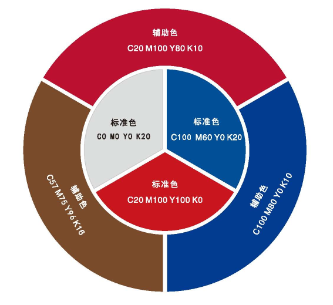
\includegraphics[height=3cm]{xjtu3.png}
  \caption{单个图形}
  \label{fig:xfig1}
\end{figure}
如果多个图形相互独立,并不共用一个图形计数器,那么用~\verb|minipage| 或者
~\verb|parbox| 就可以。否则,请参看图~\ref{fig:big1},它包含两个小图,分别是图
~\ref{fig:subfig1} 和图~\ref{fig:subfig2}。推荐使用~\verb|\subfloat|,不要再用~\verb|\subfigure|
和~\verb|\subtable|
\begin{figure}[h]
  \centering%
  \subfloat[第一个小图形]{%
    \label{fig:subfig1}
    
\includegraphics[height=3cm]{xjtu1}}\hspace{4em}%
  \subfloat[第二个小图形。如果标题很长的话,它会自动换行,这个~caption 就是这样的例子]{%
    \label{fig:subfig2}
    
\includegraphics[height=3cm]{xjtu2}}
  \caption{包含子图形的大图形}
  \label{fig:big1}
\end{figure}

古之学者必有师。师者,所以传道受业解惑也。人非生而知之者,孰能无惑?惑而不从师,
其为惑也,终不解矣。生乎吾前,其闻道也固先乎吾,吾从而师之;生乎吾後,其闻道也亦
先乎吾,吾从而师之。吾师道也,夫庸知其年之先後生於吾乎!是故无贵无贱无长无少,道
之所存,师之所存也。

嗟乎!师道之不传也久矣,欲人之无惑也难矣。古之圣人,其出人也远矣,犹且从师而问焉;
今之众人,其下圣人也亦远矣,而耻学於师。是故圣益圣,愚益愚。圣人之所以为圣,愚
人之所以为愚,其皆出於此乎?爱其子,择师而教之,於其身也,则耻师焉,惑焉。彼童子
之师,授之书而习其句读者,非吾所谓传其道、解其惑者也。句读之不知,惑之不解,或师
焉,或不焉,小学而大遗,吾未见其明也。巫医、乐师、百工之人不耻相师,  士大夫之族
曰“师”曰“弟子”之云者,则群聚而笑之。问之,则曰:彼与彼年相若也,道相似也,位
卑则足羞,官盛则近谀。呜呼!师道之不复,可知矣。巫医、乐师、百工之人。吾子不齿,
今其智乃反不能及,其可怪也欤!圣人无常师。孔子师郯子、苌子、师襄、老聃。郯子之徒,
其贤不及孔子。孔子曰:“三人行,必有我师。”是故弟子不必不如师,师不必贤於弟子。
闻道有先後,术业有专攻,如是而已。

如果要把编号的两个图形并排,那么小页就非常有用了
\begin{figure}[h]
\begin{minipage}{0.48\textwidth}
  \centering
  
\includegraphics[height=2cm]{xjtu2}
  \caption{并排第一个图}
  \label{fig:parallel1}
\end{minipage}\hfill
\begin{minipage}{0.48\textwidth}
  \centering
  
\includegraphics[height=2cm]{xjtu2}
  \caption{并排第二个图}
  \label{fig:parallel2}
\end{minipage}
\end{figure}


\subsection{定理、定义}
\begin{theorem}
宪问耻。子曰:邦有道,谷;邦无道,谷,耻也。
\end{theorem}

\begin{axiom} [论语]
君子成人之美,不成人之恶,小人反是。
\end{axiom}

\begin{definition}
君子有三戒:少之时,血气未定,戒之在色;及其壮也,血气方刚,戒之在斗;及其老也,血气既衰,戒之在得。
\end{definition}

\begin{proposition}
士不可以不弘毅,任重而道远。
\end{proposition}

\begin{lemma}
朽木不可雕也,粪土之墙不可杇也。
\end{lemma}

\begin{proof}
前不见古人,后不见来者。 
念天地之悠悠,独怆然而泪下。 
\end{proof}


\begin{assumption}
临别殷勤重寄词,词中有誓两心知。 七月七日长生殿,夜半无人私语时。 在天愿作比翼鸟,在地愿为连理枝。 天长地久有时尽,此恨绵绵无绝期。
\end{assumption}

\begin{problem}
君不见,黄河之水天上来,奔流到海不复回。君不见,高堂明镜悲白发,朝如青丝暮成雪。人生得意须尽欢,莫使金樽空对月。天生我材必有用,千金散尽还复来。
\end{problem}

\begin{conjecture}[题都城南庄]
去年今日此门中,人面桃花相映红。 人面不知何处去,桃花依旧笑春风。 
\end{conjecture}

\subsection{图文混排、高级排版}

\subsection{化学排版}

\definesubmol{a}{-P(=[::-90,0.75]O)(-[::90,0.75]HO)-}
\chemfig{[:-54]*5((--[::60]O([::-60]!aO([::-60]!aO([::60]!aHO))))<(-OH)
-[,,,,line width=2pt](-OH)>(-N*5(-=N-*6(-(-NH_2)=N-=N-)=_-))-O-)}

\subsection{绘图}

\subsection{代码、算法}

你可以通过给main.tex导言区xjtupakcages宏包添加minted选项来选择是否使用minted宏包,默认使用listings宏包。下面是各种语言书写的 hello world 在listings宏包下的效果。

C 语言版本:
\begin{lstlisting}[language={[ANSI]C}]
#inlude<stdio.h>
int main(void)	
{
    printf("Hello, World!);
    return 0;
}
\end{lstlisting}

C++版本
\begin{lstlisting}[language={[ANSI]C++}]
#include <iostream>
using namespace std;
int main()
{
  cout<<''Hello World!\n'';
  return 0;
}
\end{lstlisting}

Java 版本
\begin{lstlisting}[language={java}]
public class HelloWorld {
    public static void main(String [] args) {
        System.out.println("Hello World!");
    }
}
\end{lstlisting}

HTML 标记语言
\begin{lstlisting}[language=html]
<!DOCTYPE html>
<html>
    <body>
        Hello, world!
    </body>
</html>
\end{lstlisting}

Scala  语言:
\begin{lstlisting}%[language=scala]
object HelloWorld extends App {
  println("Hello, world!")
}
\end{lstlisting}

\subsection{bib}

this is some test\cite{IEEE-1363,Krasnogor2004e}
\section{版权声明}
声明

\section{免责声明}
声明

%================================================
%	正文后
%================================================
\backmatter

\nocite{*}
\bibliographystyle{GBT7714-2005NLang-UTF8-mod} % plain
\bibliography{ref/refs}


\appendixs{LaTeX 发行版安装及升级指南}\label{append:install}

对于初级 Windows 用户,推荐发行版本为 C\TeX{} 套装\footnote{\today 最新版本号为 2.9.2.164,},下载地址为
\begin{center}
\url{http://www.ctex.org/CTeXDownload}
\end{center}
初级用户强烈建议下载完整安装版。注意:为了避免潜在的错误,不建议把ctex安装至例如“\verb|D:\Program Files\ctex\|”的路径下\footnote{这样的文件路径中含有空格。},也不建议安装在诸如 “\verb|D:\学习工具\ctex\|”这样的路径下\footnote{这样的文件路径中含有中文。},建议安装至类似“\verb|D:\ctex\|”这样的地方。

由于本模板需要利用到一些较新的宏包,所以使用前需要对 LaTeX 进行升级,对于初级的 Windows 用户,可以通过
\begin{center}
开始 -- 所有程序 -- ctex -- MikTeX -- Maintenance(Admin) -- Update(Admin)
\end{center}
来升级,如图 \ref{fig:update} 所示。
\begin{figure}[h]
\centering
\subfloat[第一步]{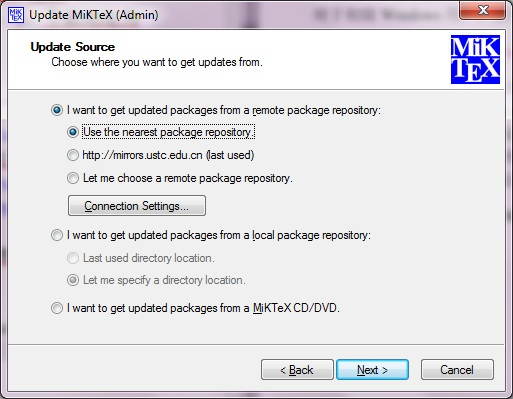
\includegraphics[width=.46\textwidth]{update1.jpg}}\quad
\subfloat[第二步]{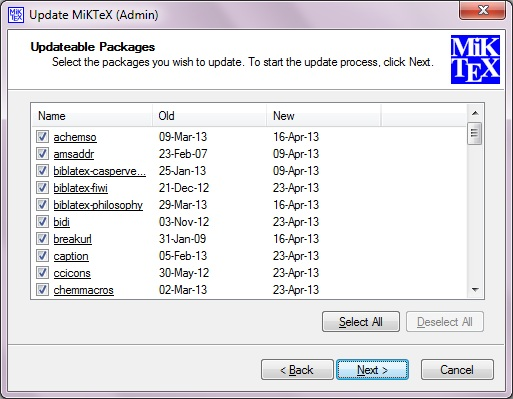
\includegraphics[width=.46\textwidth]{update2.jpg}}
\caption{C\TeX{} 套装的升级}\label{fig:update}
\end{figure}
有时,需要重复两遍上述过程。

{\color{red}\textbf{注意}},由于 C\TeX{} 套装所基于的 MikTeX 套装的问题,截止\today,上述升级完毕后会出现一个严重的问题,请一定要参考 \href{http://tex.stackexchange.com/questions/96778/a-miktex-update-removed-amsmath-as-obsolete-can-i-use-another-package-or-get-i/96795#96795}{这里}(点击查看)
修复该问题,亦即通过
\begin{center}
开始 -- 所有程序 -- ctex -- MikTeX -- Maintenance(Admin) -- Package Manager(Admin)
\end{center}
安装 \verb|amslatex-primer|、\verb|amsmath|、\verb|amscls| 三个宏包。另外对于希望使用 Times 风格的数学字体的用户,请同时安装 \verb|tex-gyre-math| 宏包。


\begin{mydenotation}
\item[HPC] 高性能计算~(High Performance Computing)
\item[cluster] 集群
\item[Itanium] 安腾
\item[SMP] 对称多处理
\item[API] 应用程序编程接口
\item[PI]	聚酰亚胺
\item[MPI]	聚酰亚胺模型化合物,N-苯基邻苯酰亚胺
\item[PBI]	聚苯并咪唑
\item[MPBI]	聚苯并咪唑模型化合物,N-苯基苯并咪唑
\item[PY]	聚吡咙
\item[PMDA-BDA]	均苯四酸二酐与联苯四胺合成的聚吡咙薄膜
\item[$\Delta G$]  	活化自由能~(Activation Free Energy)
\item [$\chi$] 传输系数~(Transmission Coefficient)
\item[$E$] 能量
\item[$m$] 质量
\item[$c$] 光速
\item[$P$] 概率
\item[$T$] 时间
\item[$v$] 速度
\item[劝  学] 君子曰:学不可以已。青,取之于蓝,而青于蓝;冰,水为之,而寒于水。
  木直中绳。(车柔)以为轮,其曲中规。虽有槁暴,不复挺者,(车柔)使之然也。故木
  受绳则直, 金就砺则利,君子博学而日参省乎己,则知明而行无过矣。吾尝终日而思
  矣,  不如须臾之所学也;吾尝(足齐)而望矣,不如登高之博见也。登高而招,臂非加
  长也,  而见者远;  顺风而呼,  声非加疾也,而闻者彰。假舆马者,非利足也,而致
  千里;假舟楫者,非能水也,而绝江河,  君子生非异也,善假于物也。积土成山,风雨
  兴焉;积水成渊,蛟龙生焉;积善成德,而神明自得,圣心备焉。故不积跬步,无以至千
  里;不积小流,无以成江海。骐骥一跃,不能十步;驽马十驾,功在不舍。锲而舍之,朽
  木不折;  锲而不舍,金石可镂。蚓无爪牙之利,筋骨之强,上食埃土,下饮黄泉,用心
  一也。蟹六跪而二螯,非蛇鳝之穴无可寄托者,用心躁也。
\end{mydenotation}


\begin{acknowledgment}
感谢党,感谢国家,感谢蛤蛤。
\end{acknowledgment}


\end{document} 
